\documentclass{article}
\usepackage{amsmath}
\usepackage{amssymb}
\usepackage{graphicx}
\usepackage{hyperref}
\usepackage[version=4]{mhchem}


\begin{document}
\section*{Problem}
( \(A M C\) ) In the obtuse triangle \(A B C, A M=M B, M D \perp B C, E C \perp B C\). If the area of \(\triangle A B C\) is 24 , find the area of \(\triangle B E D\).\\
\centering
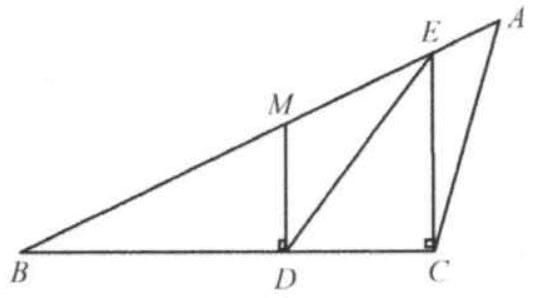
\includegraphics[width=\textwidth]{images/015.jpg}

\section*{Solution}
E.
Let \(E\) and \(F\) be the feet of the perpendicular from \(B\) and \(C\) to \(A D\). Applying\\
Pythagorean Theorem to right \(\triangle A B E, A E^{2}=A B^{2}-B E^{2}=13^{2}-12^{2}=5^{2}\). So \(A E=\) 5.

Applying Pythagorean Theorem to right \(\triangle D C F\), \(D F^{2}=D C^{2}-C F^{2}=37^{2}-12^{2}=35^{2}\). So \(D F=35\).\\
The trapezoid has area \(\frac{B C+A D}{2} \times 12=318 \Rightarrow\)\\
\centering
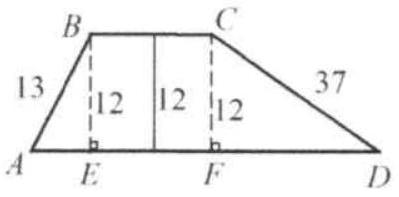
\includegraphics[width=\textwidth]{images/093(3).jpg}

\[
\begin{aligned}
& B C+A E+E F+D F=53 \\
\Rightarrow \quad & B C+5+B C+35=53 \Rightarrow \quad B C=\frac{13}{2}
\end{aligned}
\]

\end{document}
